%%%%%%%%%%%%%%%%%%%%%%%%%%%%%%%%%%%%%%%%%%%%%%%%%%%%%%%%%%%%%%%%%%%%%%%%%
\section{Experimental Evaluation}  %%%%%%%%%%%%%%%%%%%%%%%%%%%%%%%%%%%%%%
\label{rs:sec:experiments}

In practice, the comparison budget for estimating a ranking from noisy data might typically be larger than that for a single call to Quicksort, and it might not exactly match the number of comparisons required to run a given number of calls to Quicksort to completion.
Building upon the observations made at the end of Section~\ref{rs:sec:poisson}, we suggest the following practical active-learning strategy:
for a budget of $M$ pairwise comparisons, run the sorting procedure repeatedly until the budget is depleted (the last call might have to be truncated).
Then, retain only the set of $M$ comparison pairs and their outcomes and discard the rankings produced by the sorting procedure.
The final ranking estimate is then induced from the MLE over the set of $M$ comparison outcomes.

In this section, we demonstrate the effectiveness of this sampling strategy on synthetic and real-world data.
In particular, we show that it is comparable to existing AL strategies at a minuscule fraction of the computational cost.


%%%%%%%%%%%%%%%%%%%%%%%%%%%%%%%%%%%%%%%%%%%%%%%%%%%%%%%%%%%%%%%%%%%%%%%%%
\subsection{Competing Sampling Strategies}

To assess the relative merits of our sorting-based strategy, we consider three strategies that we believe are representative of the state of the art in active preference learning.

\paragraph{Uncertainty Sampling}
Developed in the context of classification tasks, this popular active-learning heuristic suggests to greedily sample the point that lies closest to the decision boundary \citep{settles2012active}.
In the context of a ranking task, this corresponds to sampling the pair of items whose relative order is most uncertain.
After $t$ observations, given an estimate of model parameters $\bm{\theta}^t$, the strategy selects the $(t\!+\!1)$-st pair uniformly at random in
\begin{align*}
\Argmin_{i \ne j} \Abs{\theta^t_i - \theta^t_j}.
\end{align*}
This set can be computed in time \BigO{N \log N} by sorting the parameters.
The parameters themselves need to be estimated, e.g., using (penalized) ML inference that in practice can be the dominating cost.

\paragraph{Bayesian Methods}
If we have access to a full posterior distribution $q^t(\bm{\theta})$ instead of a point estimate $\bm{\theta}^t$, we can take advantage of the extra information on the uncertainty of the parameters to improve the selection strategy.
A principled approach to AL consists of sampling the point that maximizes the expected information gain \citep{mackay1992bayesian}.
That is, the pair of items at iteration $t+1$ is selected in
\begin{align}
\label{rs:eq:entreduc}
\Argmax_{i \ne j} H(q^t) - \Exp{H(q^{t+1})},
\end{align}
where $H(\cdot)$ denotes the entropy function.
A conceptually similar but slightly different selection strategy is given by \citet{chen2013pairwise}.
Letting $q_{ij}$ be the marginal distribution of $(\theta_i, \theta_j)$, the pair is selected in
\begin{align}
\label{rs:eq:kldiv}
\Argmax_{i \ne j} \Exp{ \KL(q^{t+1}_{ij} \Vert q^t_{ij}) },
\end{align}
where $\KL(\cdot)$ denotes the Kullback--Leibler divergence.
Computing the exact posterior is not analytically tractable for the BT model, but a Gaussian approximation can be found in time \BigO{N^3}.
Criteria \eqref{rs:eq:entreduc} and \eqref{rs:eq:kldiv} can be computed in constant time for each pair of items.
The dominating cost is again that of estimating $\bm{\theta}$ (or, in this case, $q(\bm{\theta})$).

In addition to these existing AL strategies, we also include in our experiments a variation of our sorting-based strategy that uses Mergesort instead of Quicksort.
In the noiseless setting, Mergesort is known to use on average $\approx \num{39}~\%$ fewer comparisons than Quicksort per run \citep{knuth1998art}, but it does not benefit from the theoretical guarantees developed in Section~\ref{rs:sec:theory}.


%%%%%%%%%%%%%%%%%%%%%%%%%%%%%%%%%%%%%%%%%%%%%%%%%%%%%%%%%%%%%%%%%%%%%%%%%
\subsection{Running Time}

In this section, we briefly discuss the running time of the methods.
We implement ML and Bayesian approximate inference algorithms for the BT model as a Python library\footnote{See: \url{http://lucas.maystre.ch/choix}.}.
For approximate Bayesian inference, we use a variant of the expectation-propagation algorithm outlined by \citet{chu2005extensions}.
All experiments are performed on a server with a \num{12}-core Xeon X5670 processor running at \num{2.93}~GHz.
Numerical computations take advantage of the Intel Math Kernel Library.

We illustrate the running time of AL strategies as follows.
For $N \in \{10^2, 10^3, 10^4 \}$, we generate outcomes for $N$ comparisons pairs chosen uniformly at random among $N$ items.
For each strategy, we then measure the time it takes to select the $(N\!+\!1)$-st pair of items adaptively.
The results are presented in Table~\ref{rs:tab:runningtime}.
Note that these numbers are intended to be considered as orders of magnitude, rather than exact values, as they depend on the particular combination of software and hardware that we use.
The running time of the Bayesian AL strategies exceed \num{10} hours for $N = 10^4$ and the calls were stopped ahead of completion.
Our sorting-based methods, like random sampling, are the only AL strategies whose running time is constant for increasing $N$ (and for increasing $M$).
In fact, their running time is negligible in comparison to the other strategies, including uncertainty sampling.

\begin{table}[t]
  \caption{
Time (in seconds) to select the $(N\!+\!1)$-st pair.
Values indicated by $\varepsilon$ are below $10^{-5}$.
See text for details.
}
  \label{rs:tab:runningtime}
  \centering
  \begin{tabular}{l ccc}
    \toprule
                  & \multicolumn{3}{c}{$T$ [s]} \\
                    \cmidrule(l){2-4}
    Strategy      & $N = 10^2$      & $N = 10^3$       & $N = 10^4$ \\
    \midrule
    uncertainty   & \num{0.05}      & \num{0.5}        & \num{11}      \\
    entropy       & \num{0.3}       & \num{40}         & ---           \\
    KL-divergence & \num{0.9}       & \num{71}         & ---           \\
    Mergesort     & $\varepsilon$   & $\varepsilon$    & $\varepsilon$ \\
    Quicksort     & $\varepsilon$   & $\varepsilon$    & $\varepsilon$ \\
    random        & $\varepsilon$   & $\varepsilon$    & $\varepsilon$ \\
    \bottomrule
  \end{tabular}
\end{table}


%%%%%%%%%%%%%%%%%%%%%%%%%%%%%%%%%%%%%%%%%%%%%%%%%%%%%%%%%%%%%%%%%%%%%%%%%
\subsection{Data Efficiency}

We now investigate three datasets and measure the displacement of rankings estimated from adaptively-chosen samples, as a function of the budget $M$.
Note that in order to use uncertainty sampling and Bayesian methods, it is necessary to choose a regularization strength or prior variance in the inference step.
Different values can result in drastically different outcomes (in particular for uncertainty sampling) and, in practice, choosing a good value can be a significant challenge\footnote{Observe that our sorting-based approach is entirely parameter-free and is therefore not affected by this issue.}.
In the following, we report results for the values that worked best \emph{a posteriori}.


\paragraph{Synthetic Dataset}

We generate $N$ i.i.d. parameters $\theta_1, \ldots, \theta_n$ uniformly in $[0, (N\!+\!1) / \lambda]$ and draw samples from $\BT(\bm{\theta})$.
The ground-truth ranking is the one induced by the parameters.
Figure~\ref{rs:fig:synthetic} presents results for $N = \num{200}$ and $\lambda = \num{5}$.
In comparison to random sampling, AL is very effective and results in significantly better ranking estimates for any given number of comparisons.
The two Bayesian methods, though being the most computationally expensive, perform the best for all values of $M$, but are nearly indistinguishable from uncertainty sampling.
The two sorting-based strategies perform similarly (with a small edge for Mergesort).
They are slightly worse than the Bayesian methods but are still able to reap most of the benefits of active learning.

\begin{figure}
\centering
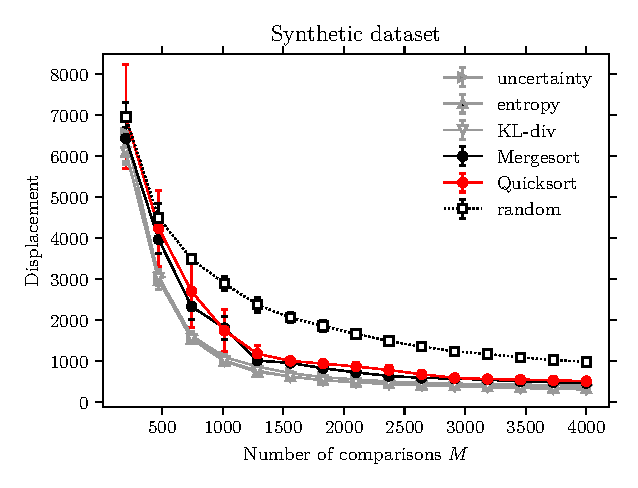
\includegraphics{rs-synthetic}
\caption{
Synthetic dataset with $\lambda = 5$ and $N = 200$.
The experiment is repeated \num{10} times, and we report the mean and the standard deviation.
Compared to random sampling, AL results in significantly better rankings for a given budget $M$.
}
\label{rs:fig:synthetic}
\end{figure}


\paragraph{Sushi Dataset}

\begin{figure}
\centering
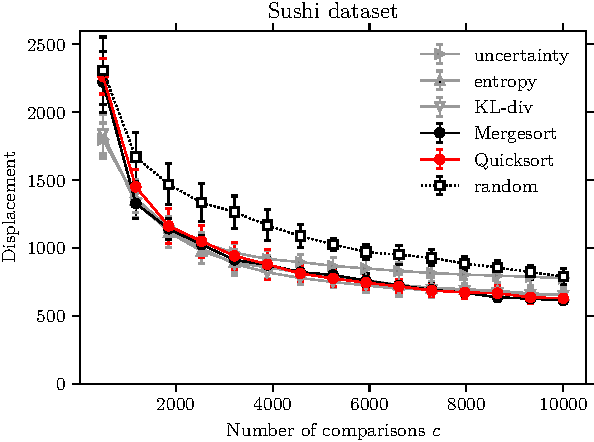
\includegraphics{rs-sushi}
\caption{
Results on two real-world datasets.
Every experiment is repeated \num{10} times, and we report the mean and the standard deviation.
Left: on the sushi dataset, sorting-based and Bayesian AL strategies have near-identical performance starting from $M \approx \num{1000}$.
Right: on the GIFGIF dataset, most AL strategies are computationally too expensive---except for sorting-based methods.
}
\label{rs:fig:sushi}
\end{figure}

Next, we consider a dataset of Sushi preferences \citep{kamishima2009efficient}.
In this dataset, \num{5000} respondents give a strict ordering over \num{10} different types of sushi.
These \num{10} sushi are chosen among a larger set of $N = \num{100}$ items.
To suit our purposes, we decompose each $10$-way partial ranking into pairwise comparisons, resulting in \num{225000} comparison outcomes.
We use all comparisons to fit a BT model that induces a ground-truth ranking\footnote{
The BT-induced ranking is almost the same as that obtained using the Copeland score.
The results are very similar if the Copeland aggregation is used as ground truth.}.

The comparisons are dense, and there is at least one comparison outcome for almost all pairs.
When an outcome for pair $(i,j)$ is requested, we sample uniformly at random over all outcomes observed for this pair.
In the rare case where no outcome is available, we return $i \prec j$ with probability $1/2$.
This enables us to compare sampling strategies in a realistic setting, where the assumptions of the BT model do not necessarily hold anymore.

Results are shown in Figure~\ref{rs:fig:sushi}.
Once again, active learning performs noticeably better than random sampling.
On this real-world dataset, the performance of our sorting-based strategies is indistinguishable from that of the Bayesian methods, after completing one entire call to the sorting procedure (slightly less than \num{1000} comparisons).
This result should be interpreted in light of the time needed to select all $10^4$ pairs: a fraction of a second for sorting-based strategies, and several hours for the Bayesian methods.
Finally, we observe that the performance of uncertainty sampling progressively degrades as $M$ increases.
A detailed analysis reveals that uncertainty sampling increasingly focuses on a small set of hard-to-discriminate pairs, symptomatic of a well-known issue \citep{settles2012active}.


\paragraph{GIFGIF Dataset}

\begin{figure}
\centering
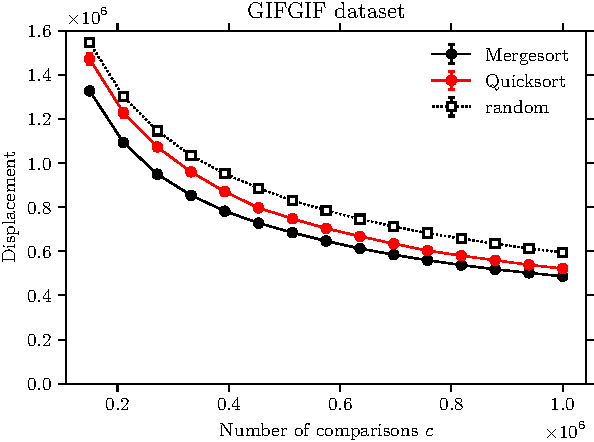
\includegraphics{rs-gifgif}
\caption{
Results on two real-world datasets.
Every experiment is repeated \num{10} times, and we report the mean and the standard deviation.
Left: on the sushi dataset, sorting-based and Bayesian AL strategies have near-identical performance starting from $M \approx \num{1000}$.
Right: on the GIFGIF dataset, most AL strategies are computationally too expensive---except for sorting-based methods.
}
\label{rs:fig:gifgif}
\end{figure}

GIFGIF\footnote{See \url{http://www.gif.gf/}.
Data available at \url{http://lucas.maystre.ch/gifgif-data}.} is a project of the MIT Media Lab that aims at explaining the emotions communicated by a collection of animated GIF images.
Users of the website are shown a prompt with two images and a question, ``Which better expresses $x$?'' where $x$ is one of 17 emotions.
The users can click on either image, or use a third option, \emph{neither}.
To date, over three million comparison outcomes have been collected.
For the purpose of our experiment, we restrict ourselves to a single emotion, \emph{happiness}; and we ignore outcomes that resulted in \emph{neither}.
We consider \num{106887} comparison outcomes over $N = \num{6120}$ items---a significant increase in scale compared to the Sushi dataset.

As the data, despite a relatively large number of comparisons, remains sparse (less than 20 comparisons per item on average), we proceed as follows.
We fit a BT model by using all the available comparisons and use the induced ranking as ground truth.
We then generate new, synthetic comparison outcomes from the BT model.
In this sense, the experiment enables us to compare sampling strategies by using a large BT model with realistic parameters.
The large number of items makes uncertainty sampling and the two Bayesian methods prohibitively expensive.
We try a simplified, computationally less expensive version of uncertainty sampling where, at every iteration, each item is compared to its two closest neighbors, but this heuristic fails spectacularly: The resulting displacement is over $5\times$ larger than random sampling for $M = 10^6$, and is therefore not reported here.

Figure~\ref{rs:fig:gifgif} compares the displacement of random sampling to that of the two sorting-based sampling strategies for increasing $M$.
The adaptive sampling approaches perform systematically better.
After $10^6$ comparisons, the displacement of random sampling is \num{14}~\% and \num{23}~\% larger than that of Quicksort and Mergesort, respectively.
Conversely, in order to reach any target displacement, Mergesort requires approximately $2 \times$ fewer comparisons than random sampling.
